
\begin{figure}
\minipage{0.40\textwidth}
  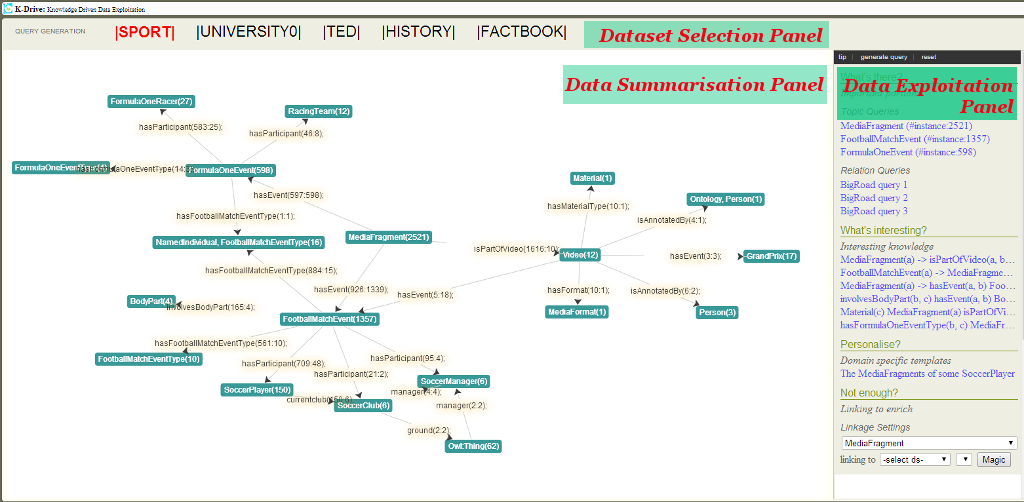
\includegraphics[scale=0.30, trim=12mm 1mm 5cm 1cm]{figures/ui_general_annotated.png}
 \caption{Data Exploitation UI}\label{fig:ui}
\endminipage\hfill
\minipage{0.50\textwidth}
  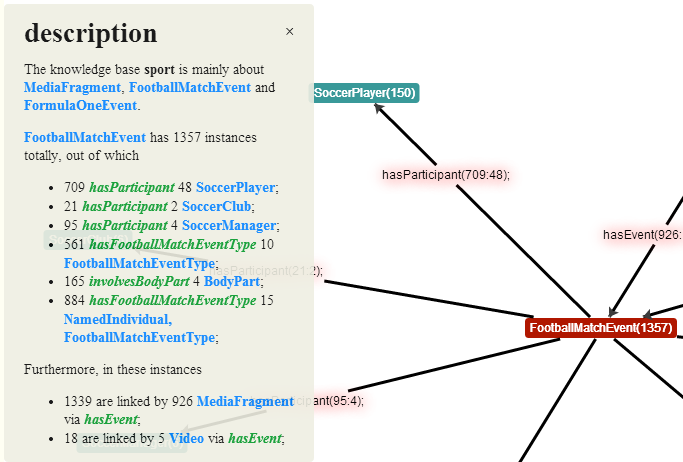
\includegraphics[scale=0.30]{figures/node.png}
  \caption{Node Browsing}\label{fig:node}
\endminipage
\end{figure}
\vspace{-2mm}
To evaluate and demonstrate the effectiveness of the summarisation in data exploitation scenarios, we implemented a summary based data exploitation system for three types of tasks i.e., gaining big picture and browsing, generating queries and enriching datasets. 

The user interface is shown in Figure~\ref{fig:ui} which contains three panels. The upper part is the \emph{Dataset Selection Panel}, which displays the list of datasets in current demo system. To switch to another dataset, one can simply click on its name in this panel. The middle panel is the main interaction and visualisation panel, the \emph{Data Summarisation Panel}. By default, it displays the summarisation of the selected dataset as an interactive graph i.e., the EDP graph. In other situations, relevant subgraphs of the EDP graph will be shown in the data exploitation process. The right panel is the \emph{Data Exploitation Panel}, which shows a bunch of UI components supporting various data exploitation operations.

Given the UI, we now demonstrate a list of data exploitation scenarios to illustrate how the summarisation can help the data exploitation tasks.

\noindent \textbf{The Big Picture and Browsing Operations}
When facing an unfamiliar dataset, users usually pursue a quick and rough \emph{big picture} of it before (s)he can assess whether it is interesting or not, e.g, what are the data describing (concepts), how are the main concepts connected to each other (relations) and which are the important parts (clusters). To help the users gain answers to these questions quickly, as shown in the \emph{Data Summarisation Panel} of Figure~\ref{fig:ui}, the EDP graph is visualised by using force-directed graph drawing techniques~\footnote{Arbor Javascript Library (\url{http://arborjs.org/introduction}) is used for the EDP graph rendering.}. Each node in the graph describes a concept. In addition to the concept name, a node is also attached with the number of instances it has in the dataset. Such statistics(c.f. Figure~\ref{fig:node}) helps to assess the importance of each concept in the dataset (in terms of data portions). The relations between (instances of) these concepts are rendered as edges, and such edges are used to calculate groups of closely related nodes, which are in turn rendered as clusters in the graph.

Two browsing operations are supported on the summary graph. The first is \emph{node browsing}. By clicking on one node in the graph, users can gain detailed description about the concept (c.f. Figure~\ref{fig:node}) including the subgraph centralised on this node which is displayed in the middle panel and the natural language description of the node displayed in a pop-up panel on the left. The second browsing operation is \emph{graph browsing}. After selecting a node, users can keep selecting/de-selecting interconnected nodes in current subgraph to grow or shrink it. This operation enables focused investigation on relations between interested nodes.

\noindent \textbf{Query Generation}
A typical usage on Semantic Web datasets is querying it. Query generation techniques~\cite{pan2013query} are helpful for either novice or advanced users because technical skills and dataset knowledge are prerequisites to write SPARQL queries. Based on the EDP summarisation, we implemented two types of query generation techniques. One is called guided query generation, which generates queries by utilising the EDP graph and statistics information attached in the graph. Such technique is good at generating queries for revealing main concepts and relations in the datasets. These two query types are called \emph{Big City Queries} and \emph{Big Road Queries} in the \emph{Data Exploitation Panel} of the system. They are analogous to big cities and highways in a geography map. The other generation technique makes use of the links in the summarisation to do efficient association rule mining~\cite{pan2013query}. This method is good at revealing insightful knowledge in the data in the form of corresponding graph patterns. Such queries are called \emph{interesting knowledge} in the system. Clicking on any of these generated queries will bring out an illustrating subgraph in the middle part of the UI.  


\noindent \textbf{Dataset Enrichment}
One of the promising features of Semantic Web techniques is the ability to link data silos to form a more valuable information space. Instead of instance-level linkage or ontology mapping, in our system, we introduce a new data linkage operation on EDPs. Such EDP-level linkage makes it possible to investigate what kinds of possibilities would be enabled after cross-dataset EDPs are linked, e.g., previously unanswerable queries might turn to be answerable by linking another dataset via EDP linkage. In the demo, we will demonstrate EDP-linkage between TED and Factbook datasets and show how such linkage can benefit a specific scenario of filtering tenders by country relations.
